In order to capture the formal use cases we will use a schema based on the one defined in Requirement Engineering Fundamentals \cite{9781937538774}.


\begin{table}[H]
    \begin{tabular}{ | >{\bfseries}l | p{8.35cm} |}
    \hline
    ID &  Unique designation of the use case \\ \hline
    Name & Unique name of the use case \\ \hline
    Priority & Importance of the use case according to applied prioritization technique \\ \hline
    Description &  Use case in user story form\\ \hline
    Dependencies & dependencies \\ \hline
    Trigger event & Name of the event that triggers this use case \\ \hline
    Actors & List of all the actors involved in this use case \\ \hline
    Preconditions & List of all necessary constraints that must be met before this use case can begin execution \\ \hline
    Posconditions & List of all states the system can be in immediately after the execution of the main scenario  \\ \hline
    Result & Description of the results that are produced during the use case execution \\ \hline
    Main scenario & Sequnce of events that occur during the use case. \\ \hline
    Alternate scenarios & Alternative sequence of events that might occur. \\ \hline

    Comments & Other infos \\ \hline
    \end{tabular}

    \caption{Use Case Template}
    \label{fig:uc_template}
\end{table}

\begin{table}[H]
    \begin{tabular}[t]{ | >{\bfseries}l | p{9.5cm} |} \hline

    ID &
        UC-1 \\ \hline
    Name &
        Capture Image \\ \hline
    Priority &
        \\ \hline
    Description &
        As a user I can capture an image of the skin lesion that I would like to have analysed. \\ \hline
    Dependencies &
        None \\ \hline
    Trigger event &
        The user activated the application and selected the "image capture" navigation item. \\ \hline
    Preconditions &
         \\ \hline
    Postconditions &
        \\ \hline
    Result &
        The captured image is saved and the system initiates the border calculation\\ \hline
    Main scenario
    &

    \begin{description}[topsep=0cm,align=left]
        \item [1.]Point the camera at the skin lesion.
        \item [2.]Rotate and move the camera until the skin lesion is centered and optimally sized.
        \item [3.]The user touches the screen to capture the image.
        \item [4.]The user is notified ( beep ) that the image has been captured
        \item [5.]The user can repeat from the begining
    \end{description}

    \\ \hline

    Alternate scenarios &
        None \\ \hline

    Comments &
        It is important that a user can capture the image with just one hand. If a lesion is located on a user's hand or arm, it's not possible to use two hands. UI should account for this if possible. \\ \hline

    \end{tabular}
  \caption{Use Case 1}
  \label{fig:uc_1}
\end{table}
\begin{table}[H]
    \begin{tabular}[t]{ | >{\bfseries}l | p{9.5cm} |} \hline

    ID &
        UC-2 \\ \hline
    Name &
        Confirm calculation of skin lesion’s border \\ \hline
    Priority &
        \\ \hline
    Description &
        As a user I want to confirm that the skin lesion’s borders have been properly calculated. \\ \hline
    Dependencies &
        UC-1 \\ \hline
    Trigger event &
        The user selected the ”confirm border” navigation item. \\ \hline
    Preconditions &
        At least one image has been captured and border calculation could complete. \\ \hline
    Postconditions &
        \\ \hline
    Result &
        After positiv confirmation, the system initiates the risk assessment calculation for the image. If the image can not be positively confirmed, the user can recapture new images ( UC-1 ) \\ \hline
    Main scenario
    &

        \begin{description}[align=left]
            \item [1.]The user is presented with a list of images.
            \item [2.]The following step is repeated for each image in the list.
            \item [3.]The user confirms that the border of the lesion has been precisely calculated.
        \end{description}

    \\ \hline

    Alternate scenarios &
        \begin{description}[align=left]
            \item [A1.] Border calculation for image has not completed.
            \item [A1.3] The user can refresh the image preview until the results of the border are visible.
            \item [A1.4] The user confirms that the border of the lesion has been precisely calculated.
        \end{description}
        \begin{description}[align=left]
            \item [A2] Border calculation is not precise or has failed.
            \item [A2.3] The user confirms that the border of the lesion has not been precisely calculated.
            \item [A2.4] The image is deleted.
        \end{description}
    \\hline

    Comments &
        \\ \hline

    \end{tabular}
  \caption{Use Case 2}
  \label{fig:uc_2}
\end{table}
\begin{table}[H]
    \begin{tabular}[t]{ | >{\bfseries}l | p{9.5cm} |} \hline

    ID &
        UC-3 \\
    \hline

    Name &
        View risk assessment \\
    \hline

    Priority &
        \\
    \hline

    Description &
        As a user I want to view the results of the risk assessment calculation. \\
    \hline

    Dependencies &
        UC-2 \\
    \hline

    Trigger event &
        The user selected the "risk assessment results" navigation item. \\
    \hline

    Preconditions &
        The system was able to complete the risk assessment calculation. \\
    \hline

    Postconditions &
        \\
    \hline

    Result &
         \\
     \hline

    Main scenario
    &

    \begin{description}[topsep=0cm,align=left]
        \item [1.]The user is presented with a list of images.
        \item [2.]The following step is repeated for each image in the list.
        \item [3.]The user can select and view and image and corresponding results in detail.

    \end{description}

    \\ \hline

    Alternate scenarios &
        \begin{description}[align=left]
            \item [A1.] Risk assessment calculation for image has not completed.
            \item [A1.3] The user can refresh the results details until the results of a risk assessment is available.
        \end{description}
    \\ \hline

    Comments &
        \\
    \hline

    \end{tabular}
  \caption{Use Case 3}
  \label{fig:uc_3}
\end{table}
\begin{table}[H]
    \begin{tabular}{ | >{\bfseries}l | p{9.5cm} |}
    \hline
    ID
    &  UC-4 \\ \hline
    Name
    & Save image and results \\ \hline
    Description
    &  As a user I want to save the image and the results of the risk assessment. \\ \hline
    Dependencies
    & UC-3 \\ \hline
    Trigger
    & The user selects the "save" navigation item. \\ \hline
    Preconditions
    & The system was able to complete the risk assessment calculation. \\ \hline
    Normal Flow
    &
    \begin{description}[align=left]
    \item [1.]The user is presented with a list of images.
    \item [2.]The can select one or more images with the corresponding risk assessment results.
    \item [3.]The user can add a title and comment.
    \item [4.]The user is presented with a confirmation that the package has been saved.
    \end{description}
    \\ \hline
    Alternate Flow
    &

    \\ \hline
    Results
    &
    A package of images and corresponding risk assessment data is stored in the archive with some metadata (title and comment).
    \\ \hline
    Comments
    &  \\ \hline
    \end{tabular}

    \caption{Use Case 4}
    \label{fig:uc_4}
\end{table}
\begin{table}[H]
    \begin{tabular}{ | >{\bfseries}l | p{9.5cm} |}
    \hline
    ID
    &  UC-5 \\ \hline
    Name
    & View archived images and data. \\ \hline
    Description
    &  As a user I want to view previously saved images and the corresponding risk assessment data. \\ \hline
    Dependencies
    & UC-4 \\ \hline
    Trigger
    & The user selects the "archive" navigation item. \\ \hline
    Preconditions
    & The system was able to complete the risk assessment calculation. \\ \hline
    Normal Flow
    &
    \begin{description}[align=left]
    \item [1.]The user is presented with a list of archived packages.
    \item [2.]The user can select an item in the list
    \item [3.]The user is presented with the images, corresponding risk assessment data and metadata for the selected item.
    \end{description}
    \\ \hline
    Alternate Flow
    &

    \\ \hline
    Results
    &
    A package of images and corresponding risk assessment data is stored in the archive with some metadata (title and comment).
    \\ \hline
    Comments
    &  \\ \hline
    \end{tabular}

    \caption{Use Case 5}
    \label{fig:uc_5}
\end{table}
\begin{table}[H]
    \begin{tabular}{ | >{\bfseries}l | p{9.5cm} |}
    \hline
    ID
    &  UC-6 \\ \hline
    Name
    & Send results to dermatologist. \\ \hline
    Description
    &  As a user I want to send a previously saved image, feature extraction data and assessment results to a dermatologist. \\ \hline
    Dependencies
    & UC-4 \\ \hline
    Trigger
    & The user selects the "archive" navigation item. \\ \hline
    Preconditions
    & The system was able to complete the risk assessment calculation. \\ \hline
    Normal Flow
    &
    \begin{description}[align=left]
    \item [1.]The user is presented with a list of archived packages.
    \item [2.]The user can select an item in the list
    \item [3.]The user can send the item as an email attachment.
    \end{description}
    \\ \hline
    Alternate Flow
    &

    \\ \hline
    Results
    &
    \\ \hline
    Comments
    &  \\ \hline
    \end{tabular}

    \caption{Use Case 6}
    \label{fig:uc_6}
\end{table}

\begin{figure}[H]
    \centering
    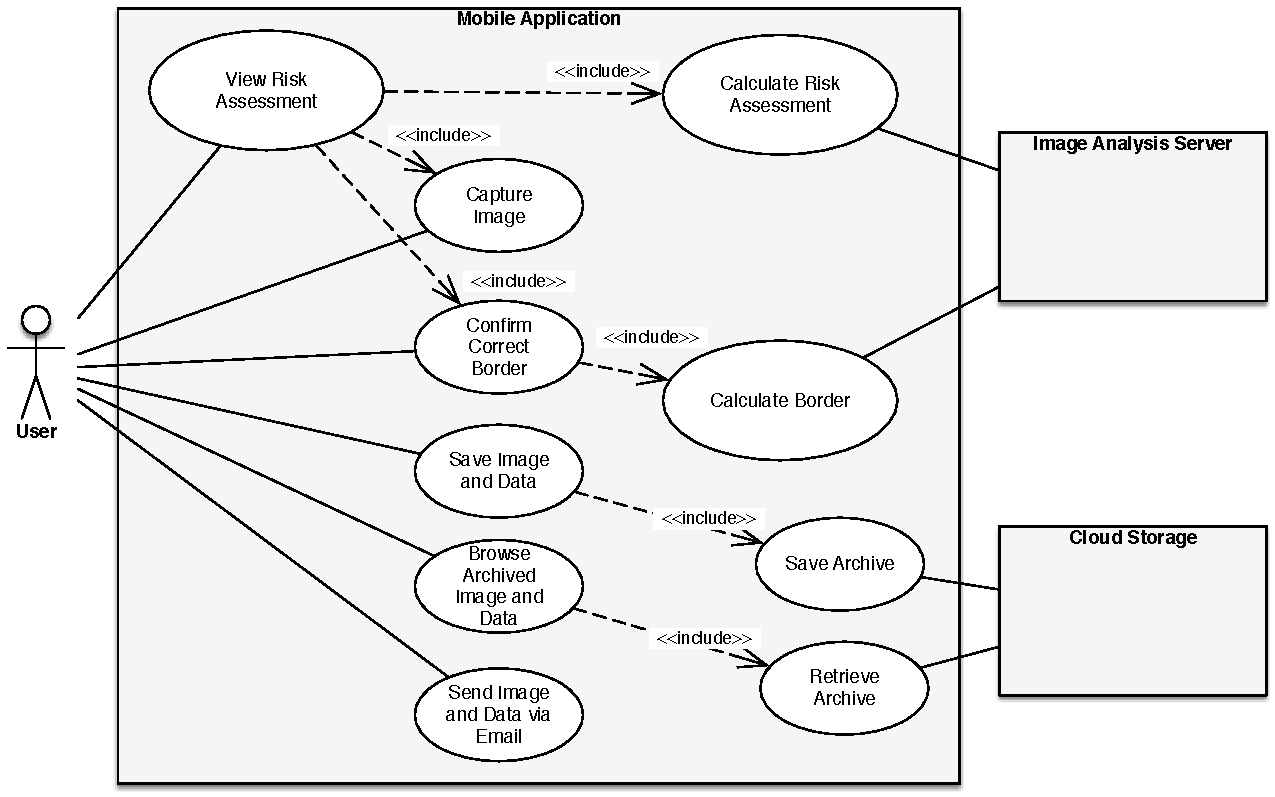
\includegraphics[height=10cm,keepaspectratio]{assets/concept/UML.pdf}
    \caption{Use Case Diagram}
    \label{fig:uml}
\end{figure}